\documentclass{beamer}
\usepackage{../../Styles/Diapo}



\newcommand{\chnum}{Chapitre 12}
\newcommand{\chtitle}{Actions et Forces}
\newcommand{\dtype}{Cours}
\newcommand{\bgcol}{blue!2!white}
\newcommand{\sectitle}{\section}

\begin{document}
\begin{frame}
    \maketitle \vspace{-2.5cm}
    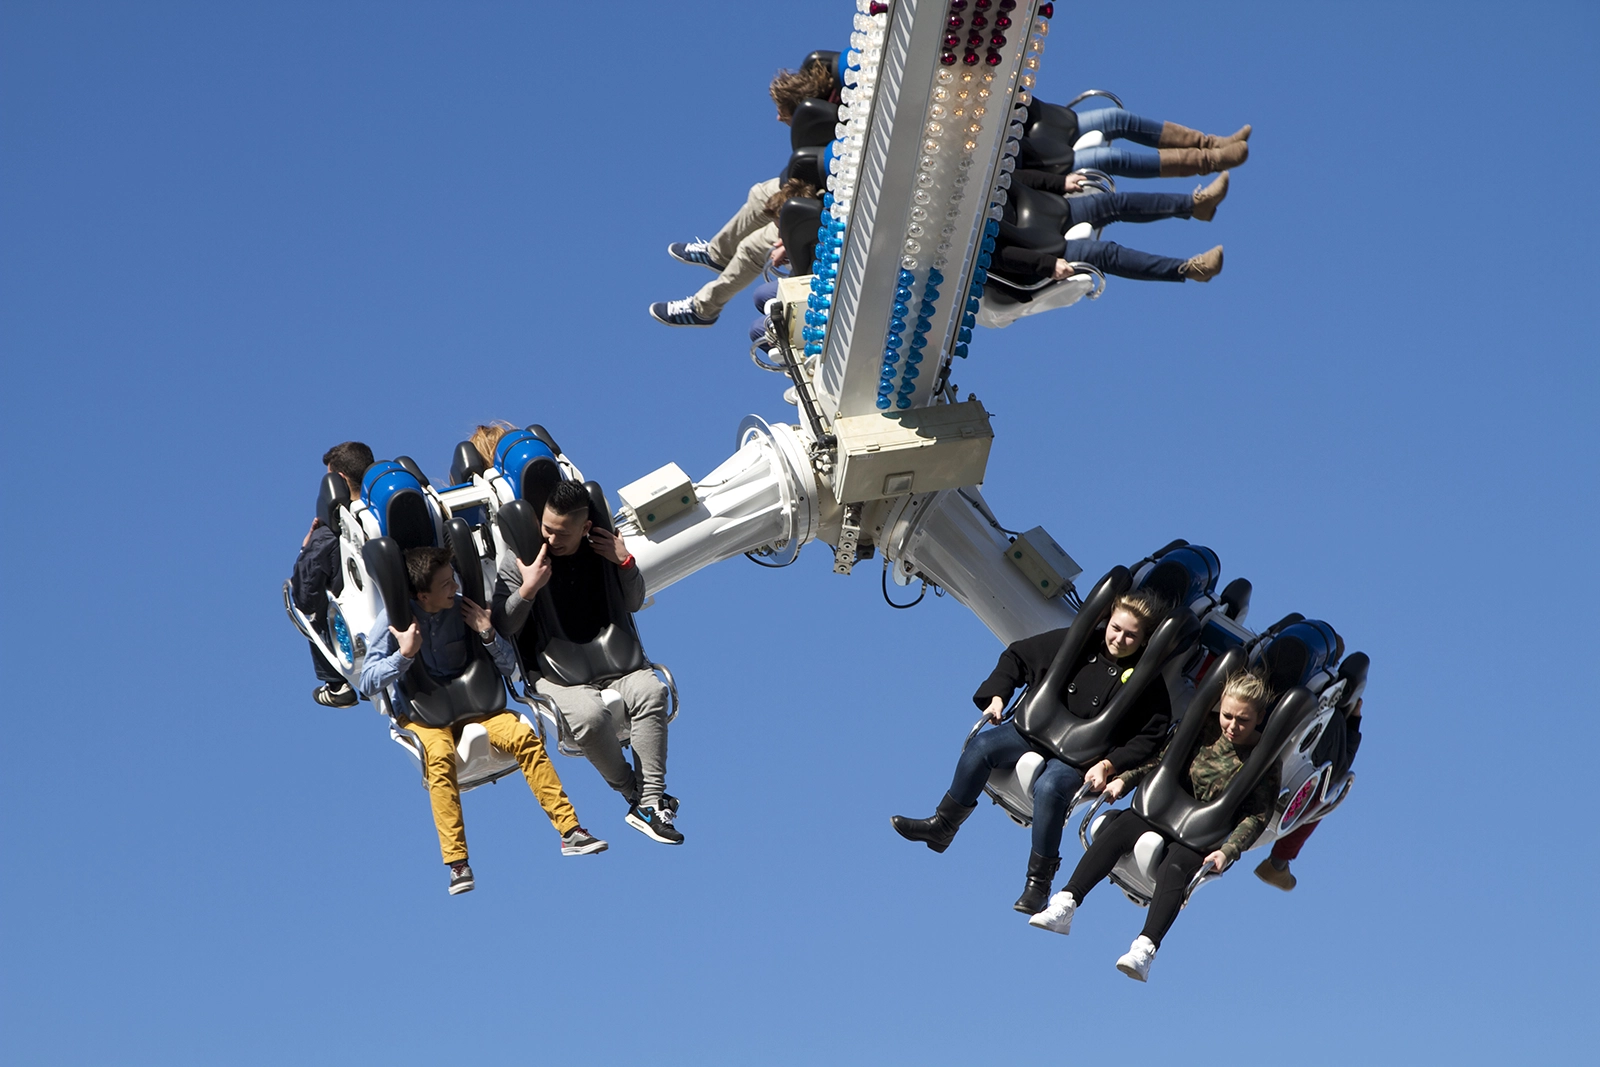
\includegraphics[width=.8\paperwidth,height=.8\paperheight]{Ressources/2GT_C6_Cours_force.png}
\end{frame}

\section{Action et forces}
\begin{frame}{Action et forces}
    \begin{minipage}[c]{.45\linewidth}
        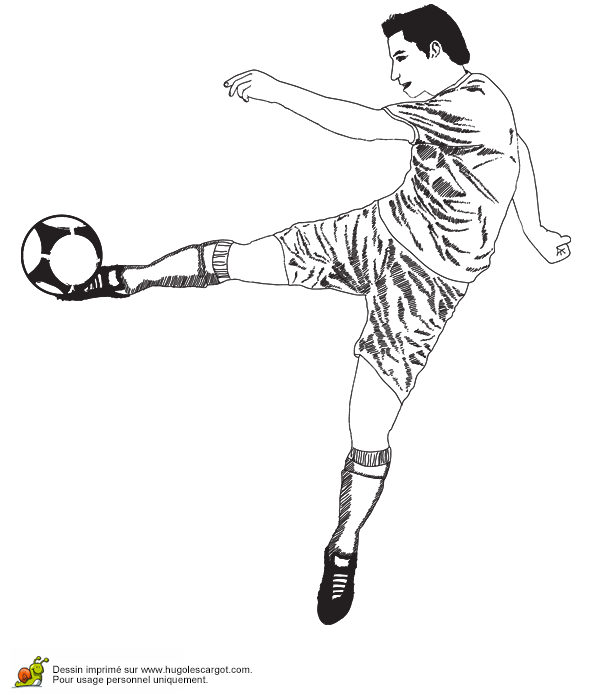
\includegraphics[scale = .3]{Ressources/2GT_C6_Cours_Fig2.png}
        \end{minipage}\begin{minipage}{.5\linewidth}
Décrire la situation suivante :\\
\pause Système étudié : le ballon
\vspace{.5cm}
\pause \large Qu'est-ce qui va agir sur le ballon ?
\pause \begin{itemize}
    \item Le pied
    \item La Terre
\end{itemize}
\pause \large Comment agissent ces systèmes extérieurs ?
\pause \begin{itemize}
    \item Le pied agit directement, au contact du ballon
    \item La Terre agit à distance, sans contact avec le ballon
\end{itemize}
\end{minipage}
\end{frame}

\subsection{Actions}
\begin{frame}{Actions}
    \colorbox{red!10}{\begin{minipage}{\linewidth}
        Lorsqu'un système 1 agit sur un système 2, on dit qu'il exerce une action.\\
	De manière \underline{réciproque} et \underline{simultanée}, le système 2 agit sur le système 1 et exerce une action.\\
	Il existe deux types d'action  de \underline{contact} ou à \underline{distance}.\\
	On utilise des \underline{diagrammes système-interactions} pour représenter l'ensemble des systèmes impliqués et représenter les actions entre le système étudié et les systèmes extérieurs.
    \end{minipage}
    }
\end{frame}

\subsection{Diagrammes système-interaction}
\begin{frame}{Diagrammes système-interaction}
\begin{minipage}[t]{.45\linewidth}
   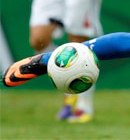
\includegraphics[scale = 1.2]{Ressources/2GT_C6_Cours_Fig1.png}
\end{minipage}
\pause[2]\begin{minipage}[t]{.45\linewidth}
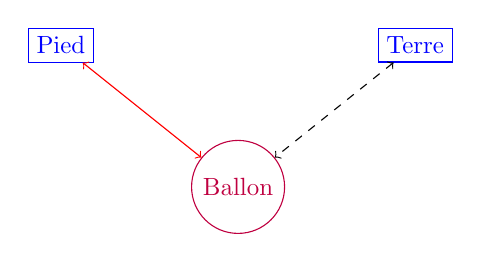
\begin{tikzpicture}[transform shape, scale=.9]
    \node[draw,rectangle, blue] (P) at (0,0){Pied};
    \node[draw,rectangle, blue] (T) at (5,0){Terre};
    \node[draw,circle, purple] (B) at (2.5,-2){Ballon};
    \draw[<->,red] (P) to (B);
    \draw[<->,black,dashed] (T) to (B);
\end{tikzpicture}
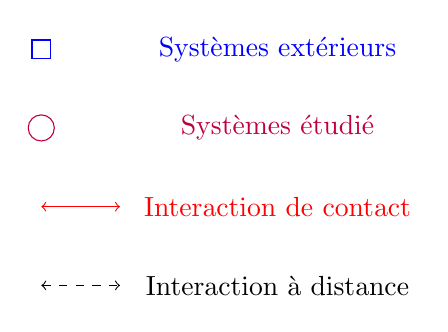
\begin{tikzpicture}
    \node[draw,rectangle, blue] (P) at (0,0){};
    \node[draw,circle, purple] (B) at (0,-1){};
    \draw[<->,red] (0,-2) to (1,-2);
    \draw[<->,black,dashed] (0,-3) to (1,-3);
    \draw[blue] (3,0) node{Systèmes extérieurs};
    \draw[purple] (3,-1) node{Systèmes étudié};
    \draw[red] (3,-2) node{Interaction de contact};
    \draw[black] (3,-3) node{Interaction à distance};
\end{tikzpicture}
\end{minipage}
\end{frame}

\subsection{Modélisation d'une action par une force}
\begin{frame}{Modélisation d'une action par une force}
    \colorbox{red!10}{\begin{minipage}{\linewidth}
        Une action exercée par un système extérieur sur le système étudié peut être modélisée par une force.\\
    Cette force est représentée par un vecteur caractérisé par :
    \begin{itemize}
        \item[$-$] Une direction
        \item[$-$] Un sens
        \item[$-$] Une norme, exprimée en Newton (\unit{\newton})
        \item[$-$] Un point d'application
    \end{itemize}
    \end{minipage}
    }
\end{frame}

\subsection{Analyse}
\begin{frame}{Analyse}
\begin{minipage}[t]{.45\linewidth}
   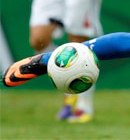
\includegraphics[scale = 1.2]{Ressources/2GT_C6_Cours_Fig1.png}
\end{minipage}

\pause[2]\begin{small}
\begin{tabular}{|>{\centering}m{1.5cm}|>{\centering}m{3cm}|>{\centering\arraybackslash}m{2.5cm}|}
\hline \rule[.5cm]{0cm}{0cm}& $\vec{P}$ & $\vv{F_{Pied/Ballon}}$\\
\hline Direction & Verticale & Horizontale\\
\hline Sens & Vers le bas & Vers la droite\\
\hline Norme & $P=m\cdot g = 4,0 N$& $F=20N$\\

\hline
\end{tabular}
\end{small}
\end{frame}

\subsection{Représentation des vecteurs}
\begin{frame}{Représentation des vecteurs}
    \begin{minipage}[t]{.5\linewidth}
    \begin{small}
    \begin{tabular}{|>{\centering}m{1.5cm}|>{\centering}m{3cm}|>{\centering\arraybackslash}m{2cm}|}
    \hline \rule[.5cm]{0cm}{0cm}& $\vec{P}$ & $\vv{F_{Pied/Ballon}}$\\
    \hline Direction & Verticale & Horizontale\\
    \hline Sens & Vers le bas & Vers la droite\\
    \hline Norme & $P=m\cdot g = 4,0 N$& $F=20N$\\
    
    \hline
    \end{tabular}
    
    \end{small}
    \end{minipage}
    
    \begin{tikzpicture}
        \draw (0,0)  node{$x$};
        \draw[->, red] (0,0) to (5,0);
        \draw[->, olive] (0,0) to (0,-1);
        \draw (2.5,0) node[above,red]{$\vv{F_{Pied/Ballon}}$};
        \draw (0,-.5) node[left,olive]{$\vec{P}$};
        
    \end{tikzpicture}
\end{frame}
    
\subsection{Exemples de cas}
    \begin{frame}{Lancer d'une balle}
    \begin{minipage}[c]{.4\linewidth}
        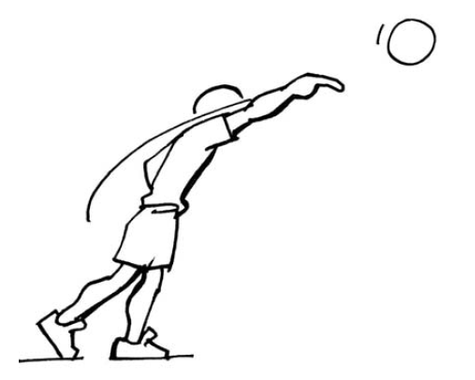
\includegraphics[scale = .4]{Ressources/2GT_C6_Cours_Fig3.png}
    \end{minipage}
    \pause \begin{minipage}[t]{.5\linewidth}
    \begin{center}
    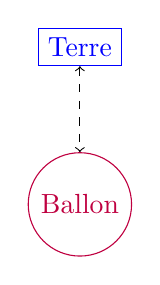
\begin{tikzpicture}
        \node[draw,rectangle, blue] (T) at (0,0){Terre};
        \node[draw,circle, purple] (B) at (0,-2){Ballon};
        \draw[<->,black,dashed] (T) to (B);
    \end{tikzpicture}
    
    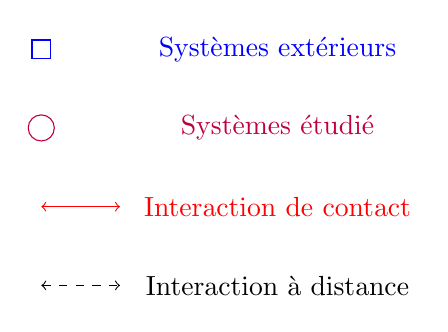
\begin{tikzpicture}
        \node[draw,rectangle, blue] (P) at (0,0){};
        \node[draw,circle, purple] (B) at (0,-1){};
        \draw[<->,red] (0,-2) to (1,-2);
        \draw[<->,black,dashed] (0,-3) to (1,-3);
        \draw[blue] (3,0) node{Systèmes extérieurs};
        \draw[purple] (3,-1) node{Systèmes étudié};
        \draw[red] (3,-2) node{Interaction de contact};
        \draw[black] (3,-3) node{Interaction à distance};
    \end{tikzpicture}
    \end{center}
    \end{minipage}
    \end{frame}
    
    \begin{frame}{Lancer d'une balle}
    \begin{minipage}[t]{.5\linewidth}
    \begin{small}
    \begin{tabular}{|>{\centering}m{2cm}|>{\centering\arraybackslash}m{3cm}|}
    \hline \rule[.5cm]{0cm}{0cm}& $\vec{P}$ \\
    \hline Direction & Verticale \\
    \hline Sens & Vers le bas \\
    \hline Norme & $P=m\cdot g = 2,0 N$\\
    
    \hline
    \end{tabular}
    
    \end{small}
    \end{minipage}
    \begin{center}
        Représentation des vecteurs :\\
        \begin{tikzpicture}
        \draw (0,0)  node{$x$};
        \draw[->, olive] (0,0) to (0,-2);
        \draw (0,-1) node[left,olive]{$\vec{P}$};
        \end{tikzpicture}
    \end{center}
    \end{frame}
    
    \begin{frame}{Objet posé}
    \begin{minipage}[c]{.4\linewidth}
       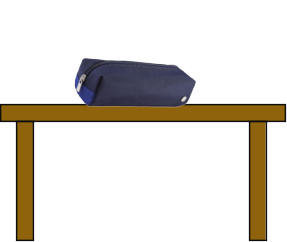
\includegraphics[scale = .4]{Ressources/2GT_C6_Cours_Fig4.png}
    \end{minipage}
    \pause \begin{minipage}[c]{.5\linewidth}
    \begin{center}
    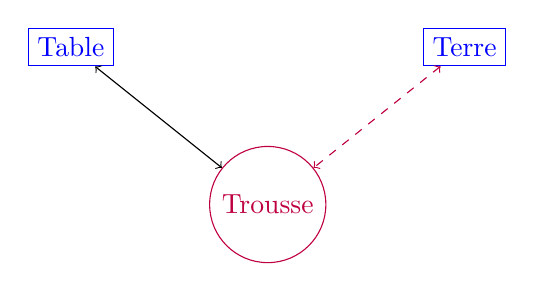
\begin{tikzpicture}
        \node[draw,rectangle, blue] (T) at (0,0){Table};
        \node[draw,rectangle, blue] (A) at (5,0){Terre};
        \node[draw,circle, purple] (B) at (2.5,-2){Trousse};
        \draw[<->,black] (T) to (B);
        \draw[<->,purple,dashed] (A) to (B);
    \end{tikzpicture}
    
    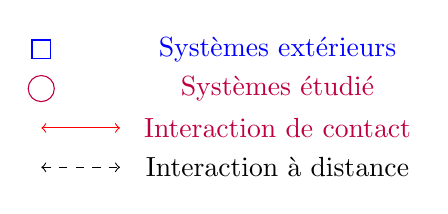
\begin{tikzpicture}
        \node[draw,rectangle, blue] (P) at (0,0){};
        \node[draw,circle, purple] (B) at (0,-.5){};
        \draw[<->,red] (0,-1) to (1,-1){};
        \draw[<->,black,dashed] (0,-1.5) to (1,-1.5);
        \draw[blue] (3,0) node{Systèmes extérieurs};
        \draw[purple] (3,-.5) node{Systèmes étudié};
        \draw[purple] (3,-1) node{Interaction de contact};
        \draw[black] (3,-1.5) node{Interaction à distance};
    \end{tikzpicture}
    \end{center}
    \end{minipage}
    \end{frame}
    
    \begin{frame}{Objet posé}
    \framesubtitle{b) Diagrammes système-interaction}
    \begin{minipage}[c]{.5\linewidth}
    \begin{small}
    \begin{tabular}{|>{\centering}m{1.5cm}|>{\centering}m{3cm}|>{\centering\arraybackslash}m{2cm}|}
    \hline \rule[.5cm]{0cm}{0cm}& $\vec{P}$ & $\vv{F_{Table/trousse}}$\\
    \hline Direction & Verticale & Horizontale\\
    \hline Sens & Vers le bas & Vers la droite\\
    \hline Norme & $P=m\cdot g = 4,0 N$& $F=4,0N$\\
    \hline
    \end{tabular}
    \end{small}
    \end{minipage}
    \begin{center}
        Représentation des vecteurs :\\
    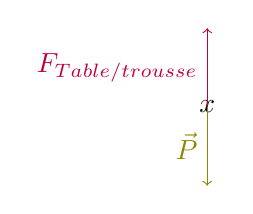
\begin{tikzpicture}
        \draw (0,0)  node{$x$};
        \draw[->, olive] (0,0) to (0,-1);
        \draw (0,-.5) node[left,olive]{$\vec{P}$};
        \draw[->, purple] (0,0) to (0,1);
        \draw (0,.5) node[left,purple]{$\vv{F_{Table/trousse}}$};
    \end{tikzpicture}
    \end{center}
    
    \end{frame}
\section{Principe des actions réciproques}
    \begin{frame}{Principe des actions réciproques}
    \begin{minipage}[c]{.85\linewidth}
    \centering
        Prenons l'exemple d'un déménageur devant déplacer une armoire :\\
        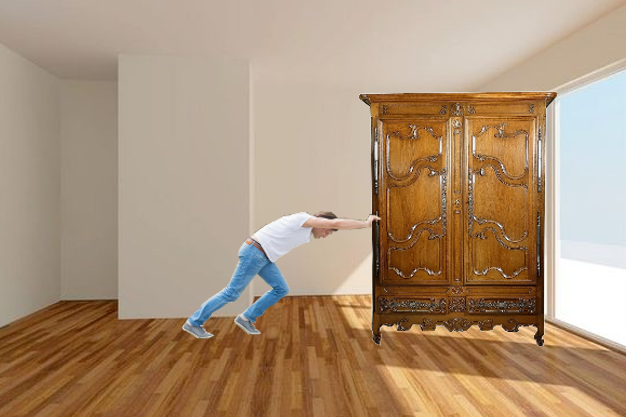
\includegraphics[width = \linewidth]{Ressources/2GT_C6_Cours_Fig5.png}
    \end{minipage}
    \end{frame}
    
    
    \begin{frame}{Principe des actions réciproques}
    \begin{minipage}[t]{.45\linewidth}
    \begin{center}
    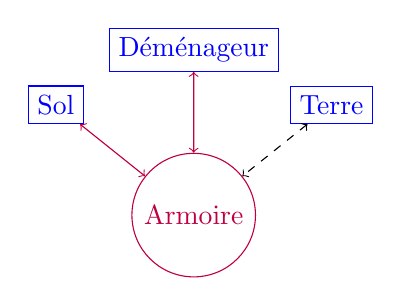
\begin{tikzpicture}[scale=.7]
        \node[draw,rectangle, blue] (S) at (0,0){Sol};
        \node[draw,rectangle, blue] (T) at (5,0){Terre};
        \node[draw,rectangle, blue] (D) at (2.5,1){Déménageur};
        \node[draw,circle, purple] (A) at (2.5,-2){Armoire};
        \draw[<->,black,dashed] (T) to (A);
        \draw[<->,purple] (S) to (A);
        \draw[<->,purple] (D) to (A);
    \end{tikzpicture}
    \vspace{.25cm}
    
    \vspace{.25cm}
    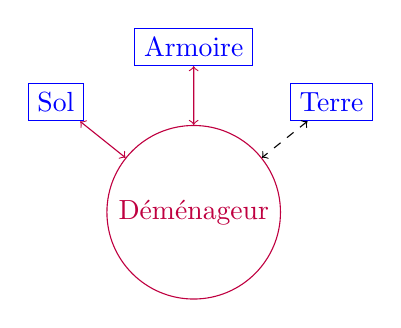
\begin{tikzpicture}[scale=.7]
        \node[draw,rectangle, blue] (S) at (0,0){Sol};
        \node[draw,rectangle, blue] (T) at (5,0){Terre};
        \node[draw,rectangle, blue] (A) at (2.5,1){Armoire};
        \node[draw,circle, purple] (D) at (2.5,-2){Déménageur};
        \draw[<->,black,dashed] (T) to (D);
        \draw[<->,purple] (S) to (D);
        \draw[<->,purple] (A) to (D);
    \end{tikzpicture}
    \end{center}
    \end{minipage}
    \end{frame}
    
    
    \begin{frame}{Principe des actions réciproques}
    \begin{minipage}[t]{.45\linewidth}
    \begin{small}
    \begin{tabular}{|>{\centering}m{1.5cm}|>{\centering}m{3cm}|>{\centering\arraybackslash}m{3cm}|}
    \hline \rule[.5cm]{0cm}{0cm}& $\vv{F_{D/A}}$ & $\vv{F_{A/D}}$\\
    \hline Direction & Horizontale & Horizontale\\
    \hline Sens & Vers le droite & Vers la gauche\\
    \hline Norme & $F_{D/A}$ = 30,0 N & $F_{A/D}$ = 30,0 N\\
    
    \hline
    \end{tabular}
    
    \end{small}
    \end{minipage}
    \end{frame}
    
    \begin{frame}{Principe des actions réciproques}
    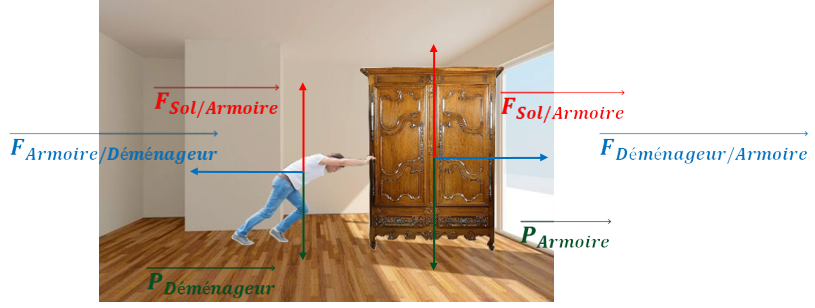
\includegraphics[scale=.35]{Ressources/2GT_C6_Cours_Fig6.png} 
    \end{frame}
    
    \begin{frame}{Principe des actions réciproques}
    \textbf{Définition :}\\
    \colorbox{red!10}{\begin{minipage}{\linewidth}
        Lorsqu'un corps A exerce une force sur un corps B, alors B exerce une force sur A telle que $\vv{F_{A/B}} = -\vv{F_{B/A}}$.\\
    La force $\vv{F_{B/A}}$ aura ainsi :
    \begin{itemize}
        \item la même direction que $\vv{F_{A/B}}$
        \item le sens opposé de celui de $\vv{F_{A/B}}$
        \item la même valeur $F_{A/B} = F_{B/A}$
    \end{itemize}
    Ce principe est également appelé la \textbf{troisième loi de Newton}.
    \end{minipage}
    }
    \end{frame}
    
\section{Exemples de forces}

\subsection{Le poids}
    \begin{frame}{Le poids}

    \begin{minipage}{.6\linewidth}
    À proximité de la surface de la Terre, tout corps de masse $m$ soumis à une force dite de pesanteur : c'est le \textbf{poids}. Le vecteur $\vec{P}$ a pour caractéristiques :
    \begin{itemize}
        \item[$-$] direction : verticale (basé sur le centre de la Terre)
        \item[$-$] sens : vers le bas (vers le centre de la Terre)
        \item[$-$] norme : $P=m\cdot g$
    \end{itemize}
    avec $P$ en Newton (N)\\
    $m$ en kilogramme (kg)\\
    $g$ est l'intensité de la pesanteur, au niveau de la mer $g$ = \num{9,81} \unit{\newton\per\kilo\gram}.
    \end{minipage}
    \begin{minipage}{.35\linewidth}
    \centering
        \begin{tikzpicture}
            \draw[line width =1.5] (-2,0) -- (2,0);
            \fill[blue!70!green!40] (0,2) circle (1);
            \draw(0,2) circle (1);
            \fill[pattern=north west lines] (-2,0) rectangle (2,-1);
            \draw[line width =1.5,-Latex, red] (0,2) to (0,.25);
            %\draw[line width =1.5,-Latex, blue] (0,1) to (0,2.75);
        \end{tikzpicture}
    \end{minipage}  
    \end{frame}
    
 \subsection{La force exercée par un support}
    \begin{frame}{Force exercée par un support}
    \begin{minipage}{.45\linewidth}
    Un corps de masse $m$, immobile et à l'horizontale, reposant sur un autre corps subit une force exercée par ce support notée $\vec{R}$.\\
    On aura alors $\vec{R} = -\vec{P}$.
    \end{minipage}
    \begin{minipage}{.45\linewidth}
        \begin{tikzpicture}
            \draw[line width =1.5] (-2,0) -- (2,0);
            \fill[blue!70!green!40,rounded corners=.2cm] (-1,0) rectangle (1,2);
            \draw[rounded corners=.2cm] (-1,0) rectangle (1,2);
            \fill[pattern=north west lines] (-2,0) rectangle (2,-1);
            \draw[line width =1.5,-Latex, red] (0,1) to (0,-.75);
            \draw[line width =1.5,-Latex, blue] (0,1) to (0,2.75);
        \end{tikzpicture}
    \end{minipage}
    \end{frame}
    
\subsection{Force exercée par un fil}
    \begin{frame}{Force exercée par un fil}
    \begin{minipage}{.45\linewidth}
    Un corps de masse $m$, suspendu par un fil non extensible, subit une force exercée par le fil notée $\vec{T}$, telle que $\vec{T}=-\vec{P}$.
    \end{minipage}
    \begin{minipage}{.45\linewidth}
    \centering
        \begin{tikzpicture}
            \fill[blue!70!green!40,rounded corners=.2cm] (-1,0) rectangle (1,2);
            \draw[rounded corners=.2cm] (-1,0) rectangle (1,2);
            %\fill[pattern=north west lines] (-2,0) rectangle (2,-1);
            \draw[line width =1.5] (0,1.75) -- (0,4);
            \draw[line width =1.5,-Latex, red] (0,1) to (0,-.75);
            \draw[line width =1.5,-Latex, blue] (0,1) to (0,2.75);
        \end{tikzpicture}
    \end{minipage}
    \end{frame}

 \subsection{Force d'interaction gravitationnelle}
    \begin{frame}{Force d'interaction gravitationnelle}
    \begin{minipage}{\linewidth}
    \small
    On considère en deux points différents de l'espace, deux objets $A$ et $B$, de masses respectives $m_A$ et $m_B$.\\
    On note la distance qui les sépare $d$.\\
    Ces deux corps vont exercer une attraction mutuelle telle que $\vv{F_{A/B}} = -\vv{F_{B/A}}$.\\
    Cette force d'interaction gravitationnelle aura les caractéristiques suivantes :
        \begin{itemize}
            \item[$-$] Direction : donnée par la droite reliant le centre des corps $A$ et $B$
            \item[$-$] Sens : $\vv{F_{A/B}}$ de $B$ vers $A$ et  $\vv{F_{B/A}}$ de $A$ vers $B$
            \item[$-$] Norme : $F_{A/B} = F_{B/A} = G\cdot \dfrac{m_A\cdot m_B}{d^2}$ 
        \end{itemize}
    Avec $m_A$ et $m_B$, les masses de $A$ et $B$ en kilogrammes (\unit{kg})\\
    $d$ la distance entre $A$ et $B$ en mètre (\unit{\meter})\\
    $G$ la constante de gravitation universelle $G = \SI{6,67E-11}{\newton\per\meter\squared\per\kilo\gram\squared}$
    \end{minipage}
    
    \end{frame}
    
    \begin{frame}{Force d'interaction gravitationnelle}
    \begin{minipage}{\linewidth}
    \centering
        \begin{tikzpicture}
            \draw [fill=gray!50,rounded corners = .3cm] (0,0) -- (0,1.5) -- (1,1) -- (1,0) -- cycle;
    
            \draw [fill=gray!50,decorate, rounded corners=0.2cm] (6,0) -- (6,-1) -- (5,-2) -- (5,-1) -- cycle;
    
            \node[above] (A) at (.5,.65){$A$};
            \node[above] (B) at (5.5,-1){$B$};
            \node (d) at (3,.65){$d$};
            
            \draw(.5,.65) node{$\times$};
            \draw(5.5,-1) node{$\times$};
    
            \draw[-Latex,red,line width=1] (.5,.65) to (2,.14);
            \draw[-Latex,blue,line width=1] (5.5,-1) to (4,-.52);
    
            \draw[Latex-Latex,purple,line width=1,dashed] (.5,1.15) to (5.5,-.5);
    
            \draw[red](.75,-.5) node{$\vv{F_{B/A}}$};
            \draw[blue](4.5,-1.5) node{$\vv{F_{A/B}}$};
    
            \draw(.5,1.5) node{$m_A$};
            \draw(5.5,-2) node{$m_B$};
            
            %\draw(0,-2) grid(6,3);
        \end{tikzpicture}
    \end{minipage}
    \end{frame}
    
\section{Le principe d'inertie}

    \subsection{Effet d'une force exercée sur le mouvement d'un système}
\begin{frame}{Effet d'une force exercée sur le mouvement d'un système}
    
            Une force s'exerçant sur un système peut modifier la valeur de sa vitesse et/ou la direction du mouvement de ce système. Elle peut donc modifier le vecteur vitesse $\vec{v}$ de ce système.\\
            \textbf{Principe d'inertie}\\
            Lorsque les forces qui s’appliquent sur un système se compensent, le vecteur vitesse $\vec{v}$ ne varie pas. Le mouvement est donc au repos ($\vec{v}=\vec{0}$) ou rectiligne et uniforme ($\vec{v}=\vec{cst}$)\\
            
            \textbf{Contraposée du principe d'inertie}\\
            Lorsque, entre deux instants voisins, le vecteur vitesse d’un système varie, alors les forces qui s’exercent sur lui ne se compensent pas.
\end{frame}

\subsection{La variation du vecteur vitesse}
\begin{frame}{La variation du vecteur vitesse}
            Au cours de la trajectoire, si l’une des trois caractéristiques du vecteur vitesse change (valeur, direction ou sens), la contraposée du principe d’inertie permet de déduire que les forces exercées sur l’objet ne se compensent pas. Inversement, si le vecteur vitesse est invariant lors du mouvement, les forces appliquées au système se compensent.
\end{frame}

\subsection{La chute libre verticale}
\begin{frame}{La chute libre verticale}
        La chute libre est définie lorsqu’un système n’est soumis qu’à son poids $\vec{P}$.
        Dans le cas d’une chute libre verticale, le vecteur vitesse va varier entre deux instants voisins. On peut donc en conclure que le mouvement n’est pas rectiligne et uniforme. De plus, on constate que la direction et le sens du vecteur variation de vitesse $\Delta \vec{v}= \vv{v_{i+1}} - \vec{v_{i}}$ sont identiques à ceux du poids.
\end{frame}
\end{document}